\begin{sectionbox}[Problem]\nospacing
  Picking the nex point greedily by maximizing the mean payoff\cref{defn:pure_exploration_follow_the_leader}
  \begin{align}
    x_{t}=\argmax_{x\in D}\mean_{t-1}(x)
  \end{align}
  of the posterior distribution tends to lead to local optima.
\end{sectionbox}
\begin{sectionbox}[Assumption]\nospacing
  If the true function $f$ is within the confidence bounds of our posterior distribution:
  \begin{align*}
    f(x)\in(\mean(x)-\betac\std,\mean(x)+\betac\std)
  \end{align*}
  then it follows that:
  \begin{align}
    f\left(\xvec^{*}\right)\geq\max\mean(x)-\betac\std(x)\label{eq:gp-ucp-lcb}
  \end{align}
  this implies that we should focus only on certain regions.
  Because if the best predicted value of a point $\mean(x')+\std(x')$ is less
  then the \textit{best lower confidence bound}\cref{eq:gp-ucp-lcb} then the maximum cannot be at $x'$:
  \begin{align}
    f\left(\xvec^{*}\right)\geq\max\mean(x)-\betac\std(x)\geq\mean(x')+\std(x')
  \end{align}
  \todo[inline]{add own figure}
  \begin{figure}[H]
    \centering
    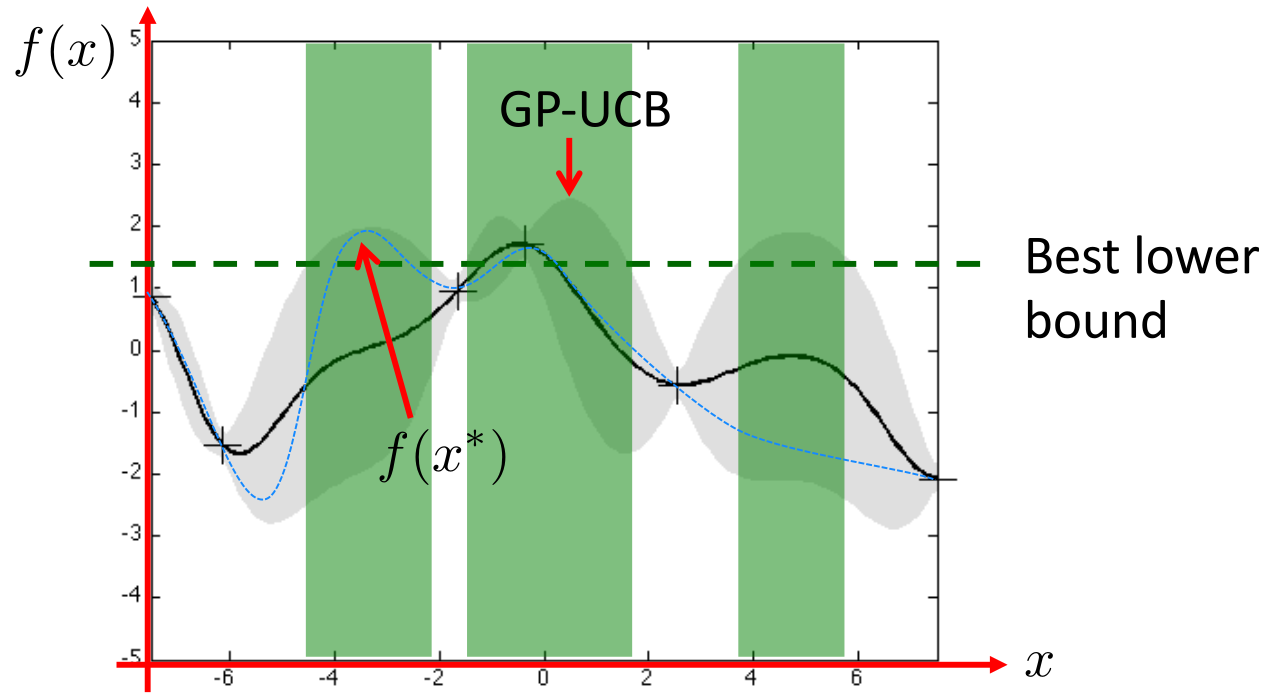
\includegraphics[width=1.0\textwidth]{src/bayesian_optimization/figures/gp-ucb.png}
  \end{figure}
  This idea can be utilized in various ways:
  \begin{itemizenosep}
    \item GP-UCB \cref{subsubsec:gaussian_process-ucb}
    \item Thompson Sampling \cref{subsubsec:thompson_sampling}
  \end{itemizenosep}
\end{sectionbox}
%%% Local Variables:
%%% mode: latex
%%% TeX-command-extra-options: "-shell-escape"
%%% TeX-master: "../../../formulary"
%%% End:
